\chapter{General State of the Art}


\section{Context}

To replace materials that are very practical but very problematic for our environment, convince people of the usefulness of the replacement. on the one hand, by making functional objects. But also by opening the door to new imaginations that broaden the scope of what's possible. that's why, in the same way as classical research, design helps to shape this problem. 
\begin{marginfigure}[-5cm] % Adjust the vertical placement
    \centering
    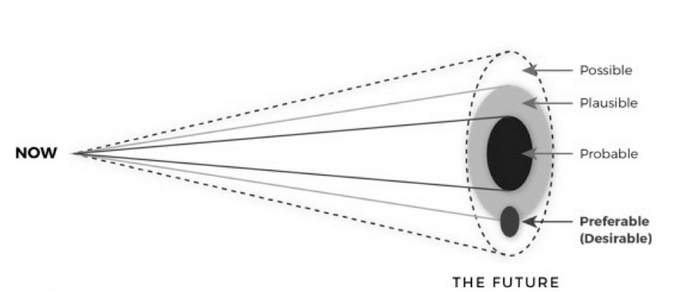
\includegraphics[width=\linewidth]{images/futures_cone.png}
    \caption{futures cone representation}
    \label{fig:plastics}
\end{marginfigure}
Science in this field relatively new. The starting point differs depending on how define biomaterials and how make, or rather grow them. 
More globally, biomaterials are at the crossroads of many fields of scientific and even artistic research. From agriculture to design, from synthetic biology to fashion, from DIY fermented drink to biohacking in the kintchen\cite{CiteTheOdin}.
This is in line with new interdisciplinary courses integrating biodesign, such as MIT's "How To Grow (Almost) Anything" course\cite{CiteMITHTGAA}. 

As matter of fact, the starting point might be the first crops domestication. At this time the goal was only to produce food, and the process were optimized by selective breeding. By taking the plants with the biggest fruit or the best resistance to environment, from generation to generation plants were "optimized" for the population.
Besides, the use of wood are very use in numerous sectors\cite{ramage2017wood} push by international directive of less CO2 emmission and waste. 
  
However, today, biomaterials or biobased materials in this study are more in line with the aim of replace existing materials like plastics.
This biomaterials production projects are aimed to create in the futures of cone plausible or possible futures. 
Moreover the development of this new materials go hand in hand with the evolution of new machines for biomaterials. Bioreactors are controlled environment systems. There is no notable differences in hardware part from bioreactors in the litterature. The general form is a isolated space from outside environmental conditions, 
combine with a controler responsible of sensors and actuator (i.e :fogger, fan, thermal resistance...). The controler is also responsible to send data when monitoring is wanted. All powered by energy from different sources. 

A review 


\paragraph[short]{Industry} 
ecovative mycoworks 

\paragraph[short]{In Design} 

suzane lee biofabricate 




\section{Biomaterial}
\subsection{S.C.O.B.Y Lether} 


\subsection{Mycelium}


\subsection{Other Biomaterial}




















\section{Bioreactor \& Controlled Environment }

\subsection{Controlled Environment} 



















\subsection{Bioreactor}
\subsection{Bioreactor Mycelium}
\subsection{Bioreactor S.C.O.B.Y}


\section{Discution and limitation}